\section{Trigger} 
\label{sec:trigger}

Events for the signal region are collected using a set of dedicated
triggers designed to select events with large $\ptmiss$ and large $\mht$ based on
the online particle flow (PF) algorithm. In these dedicated trigger algorithms,
identified PF muons are removed from the event before the
$\ptmiss$ and the $\mht$ objects are calculated. With this definition,
the signal trigger paths can also be used to select single and double muon events for the W and Z control regions, respectively.

Electron events for the W and Z regions are selected using a single electron trigger.
To ensure the trigger efficiency also for high-$\pt$ electrons, the single electron trigger is used in combination with
a single photon trigger~\cite{CMS-EGM-TWIKI-HLT}. The same photon trigger is used to select events for the photon control region.

The full list of triggers used, along with the L1 seeds and the associated primary datasets are shown in Table~\ref{tab:triggers}.
\begin{table}[h]
    \centering
    \def\arraystretch{1.5}

    \small
    \caption{HLT paths and the associated L1 seeds used in the analysis for the 2017 and 2018 datasets. 
    The HLT paths ending in ``\_HT60'' are backup triggers introduced to mitigate noise rate problems in 2017. 
    Their inclusion is not strictly necessary for 2018, but is done for consistency.}

    \footnotesize
    \begin{tabular}{l l c c}
        \hline\hline
        Year                   & HLT path                                                  & L1 seed                         & Primary dataset               \\\hline\hline
        \multirow{5}{*}{2017}  & HLT\_PFMETNoMu120\_PFMHTNoMu120\_IDTight                  & \texttt{L1\_ETMHF70}            & MET                           \\
                               & HLT\_PFMETNoMu120\_PFMHTNoMu120\_IDTight\_PFHT60          & \texttt{L1\_ETMHF80\_HTT60er }  & MET                           \\\cline{2-4}
                               & HLT\_Ele35\_WPTight\_Gsf                                  & \texttt{L1\_SingleEG24}         & SingleElectron                \\\cline{2-4}
                               & \multirow{3}{*}{HLT\_Photon200}                           & \texttt{L1\_SingleEG30}         & \multirow{3}{*}{SinglePhoton} \\
                               &                                                           & \texttt{L1\_SingleJet170}       &                               \\
                               &                                                           & \texttt{L1\_SingleTau100er2p1}  &                               \\\hline\hline

        \multirow{11}{*}{2018} & \multirow{2}{*}{HLT\_PFMETNoMu120\_PFMHTNoMu120\_IDTight} & \texttt{L1\_ETMHF100}           & \multirow{3}{*}{MET}          \\
                               &                                                           & \texttt{L1\_ETM150}             &                               \\
                               & HLT\_PFMETNoMu120\_PFMHTNoMu120\_IDTight\_PFHT60          & \texttt{L1\_ETMHF90\_HTT60er}   &                               \\\cline{2-4}
                               & \multirow{3}{*}{HLT\_Ele32\_WPTight\_Gsf}                 & \texttt{L1\_SingleIsoEG24er2p1} & \multirow{3}{*}{EGamma}       \\
                               &                                                           & \texttt{L1\_SingleEG26er2p5}    &                               \\
                               &                                                           & \texttt{L1\_SingleEG60}         &                               \\\cline{2-4}

                               & \multirow{5}{*}{HLT\_Photon200}                           & \texttt{L1\_SingleEG34er2p5}    & \multirow{5}{*}{EGamma}       \\
                               &                                                           & \texttt{L1\_SingleJet160er2p5}  &                               \\
                               &                                                           & \texttt{L1\_SingleJet180}       &                               \\
                               &                                                           & \texttt{L1\_SingleTau120er2p1}  &                               \\
                               &                                                           & \texttt{L1\_SingleEG60}         &                               \\\hline

        \hline\hline %--------------------------------------------------------------------------------------------------------------------------      \
    \end{tabular}

    \label{tab:triggers}
\end{table}

\subsection{Efficiency measurement}

The performance of $\ptmiss + \htmiss$ based triggers is measured by using single muon events, i.e. sample enriched in
$W \rightarrow \mu\nu$ decays. The measurement is performed by using both data and MC samples for 2017 and 2018, seperately.

$W \rightarrow \mu\nu$ events are selected from Single Muon dataset and WJetsToLNu MC sample. 
The muon must must pass the tight ID requirement. In addition, the transverse mass of the muon must not exceed $160 \ GeV$. 
There should be no additional leptons or photons and b-jets identified in the event. In addition, there must be at least 
two jets in the event, and the leading two jets must have $\pt$ higher than $80 \ GeV$ and $40 \ GeV$, respectively. 
Finally, the two leading jets must satisty $\detajj > 1.0$ and $\dphijj < 1.5$.

To understand the dependence of the efficiencies on the jet kinematics, we measured the efficiency in three different categories:

\begin{itemize}
    \item Two central VBF jets: Leading two jets both satisfying $|\eta| \leq 2.4$
    \item Two forward VBF jets: Leading two jets both satisfying $|\eta| > 2.4$
    \item One central and one forward VBF jet: One of the leading jets is central with $|\eta| \leq 2.4$ and the other jet in the pair is forward 
    with $|\eta| > 2.4$
\end{itemize}

In these three categories, efficiencies are measured as a function of $\mjj$ and recoil, using both data and MC samples for 2017 and 2018,
seperately. Figs.~\ref{fig:eff_mjj_2017_1m}, \ref{fig:eff_mjj_2018_1m}, \ref{fig:eff_recoil_2017_1m} and \ref{fig:eff_recoil_2018_1m} show 
the results. 

Fig.~\ref{fig:eff_mjj_2017_1m} shows the efficiencies as a function of $\mjj$ in data and MC for the three categories in 2017, 
whereas Fig.~\ref{fig:eff_mjj_2018_1m} shows the efficiencies as a function of $\mjj$ in data and MC for the three categories in 2018. 
Fig.~\ref{fig:eff_recoil_2017_1m} shows the efficiencies as a function of recoil in data and MC for the three categories, 
for 2017 samples, whereas Fig.~\ref{fig:eff_recoil_2018_1m} shows the efficiencies as a function of recoil in data and MC 
for the three categories, for 2018 samples. 

\begin{figure}[htp]
    \begin{center}
        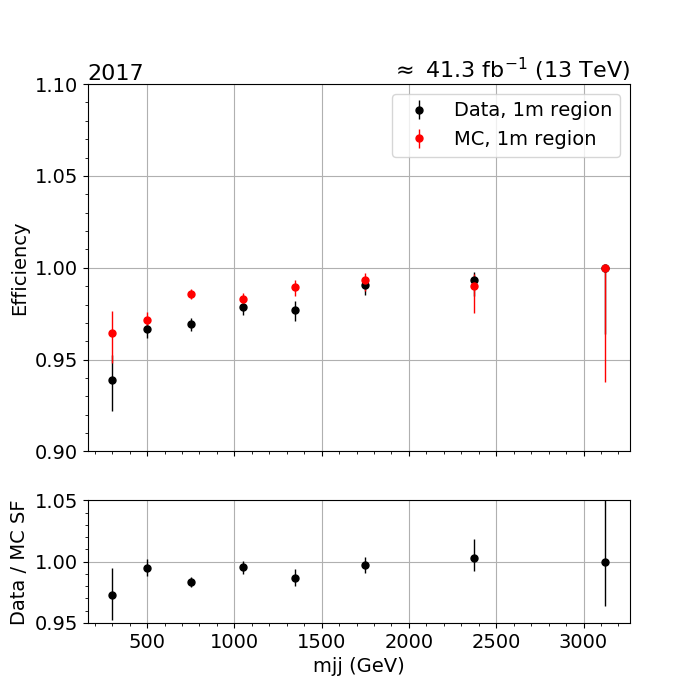
\includegraphics[width=0.49\textwidth]{fig/efficiency/trigger/met/mjj/data_mc_comparison_1m_2017_one_jet_forward_one_jet_central.png}
        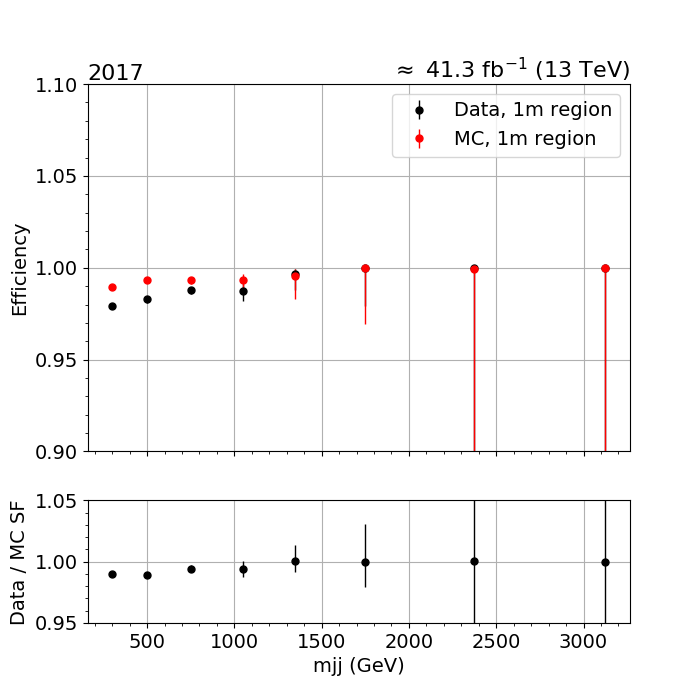
\includegraphics[width=0.49\textwidth]{fig/efficiency/trigger/met/mjj/data_mc_comparison_1m_2017_two_central_jets.png} \\
        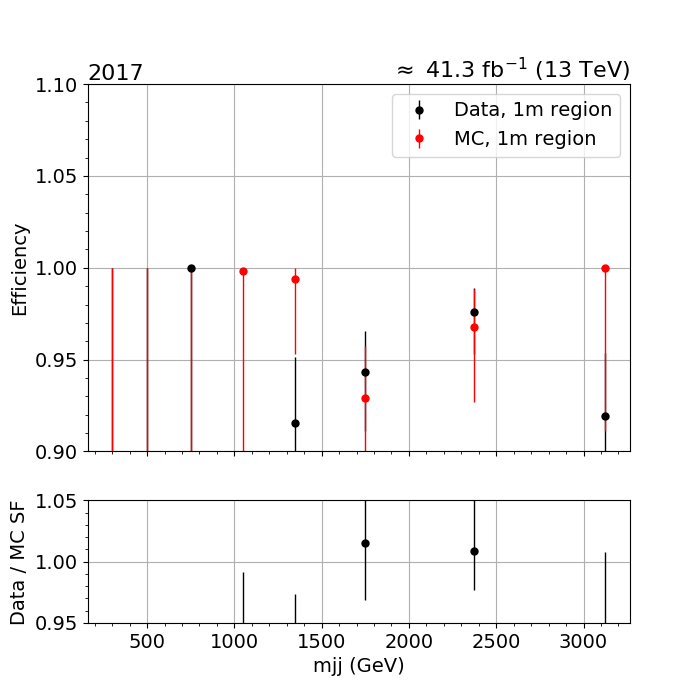
\includegraphics[width=0.49\textwidth]{fig/efficiency/trigger/met/mjj/data_mc_comparison_1m_2017_two_forward_jets.png}
    \end{center}
    \caption{MET trigger efficiency as a function of mjj in three categories: One forward jet and one central jet, two central jets and
            two forward jets. These results are obtained from 2017 data and MC samples with the selection of single muon events.} 
    \label{fig:eff_mjj_2017_1m}      
\end{figure}

\begin{figure}[hbp]
    \begin{center}
        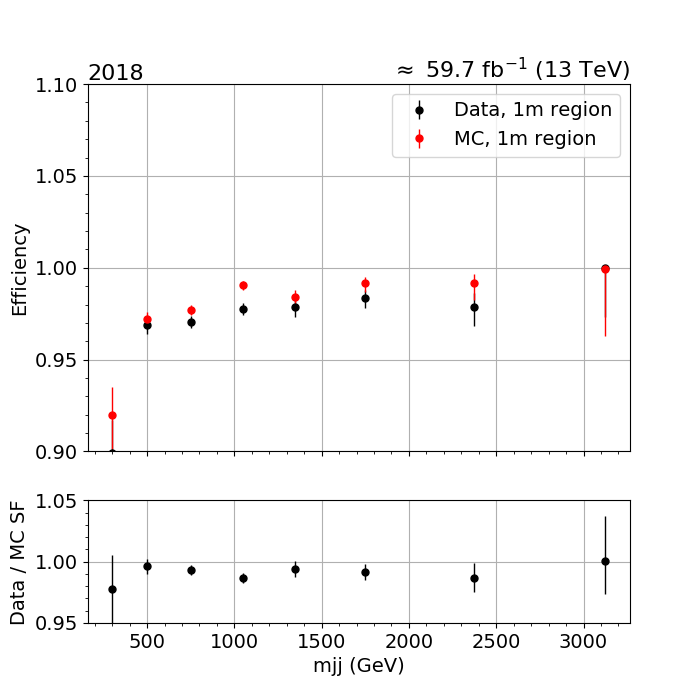
\includegraphics[width=0.49\textwidth]{fig/efficiency/trigger/met/mjj/data_mc_comparison_1m_2018_one_jet_forward_one_jet_central.png}
        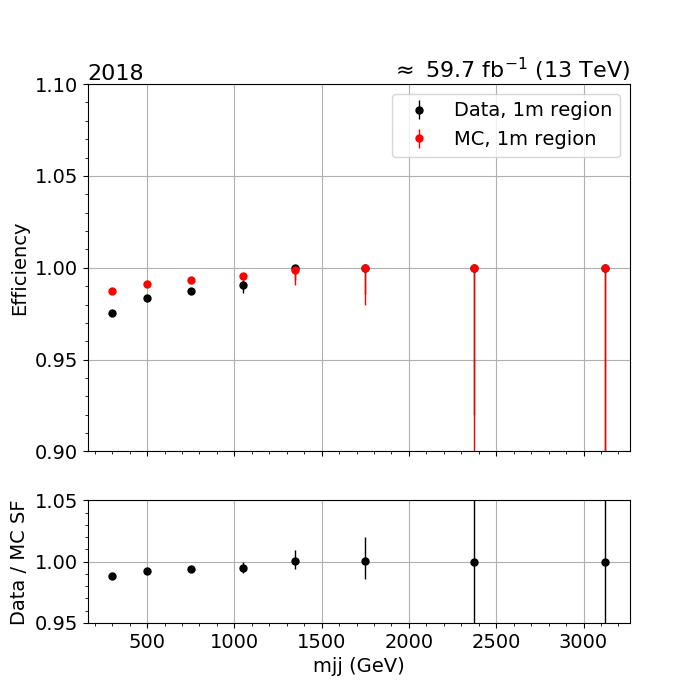
\includegraphics[width=0.49\textwidth]{fig/efficiency/trigger/met/mjj/data_mc_comparison_1m_2018_two_central_jets.png} \\
        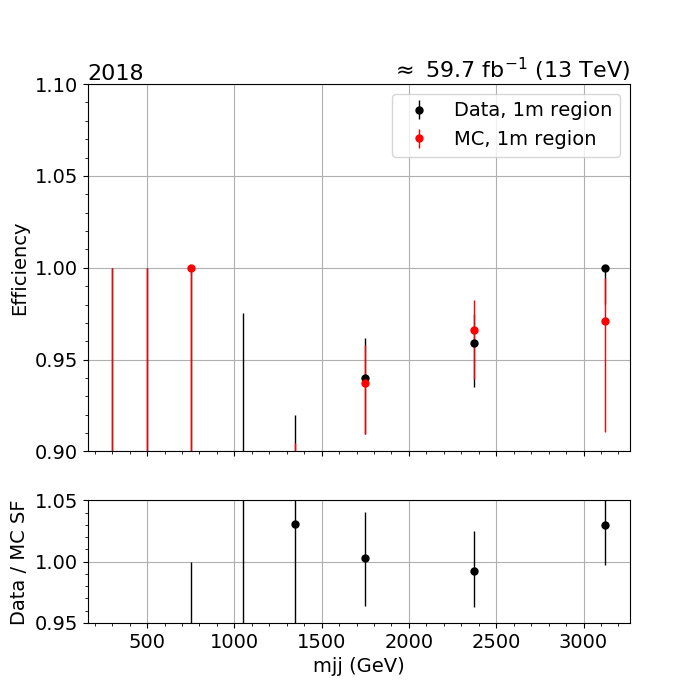
\includegraphics[width=0.49\textwidth]{fig/efficiency/trigger/met/mjj/data_mc_comparison_1m_2018_two_forward_jets.png}
    \end{center}
    \caption{MET trigger efficiency as a function of mjj in three categories: One forward jet and one central jet, two central jets and
            two forward jets. These results are obtained from 2018 data and MC samples with the selection of single muon events.}   
    \label{fig:eff_mjj_2018_1m}
\end{figure}

\begin{figure}[htp]
    \begin{center}
        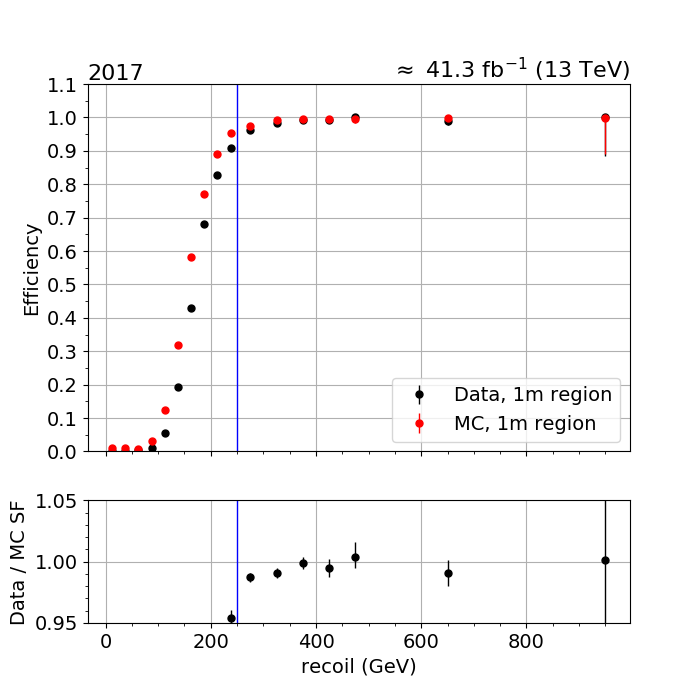
\includegraphics[width=0.49\textwidth]{fig/efficiency/trigger/met/recoil/data_mc_comparison_1m_2017_one_jet_forward_one_jet_central.png}
        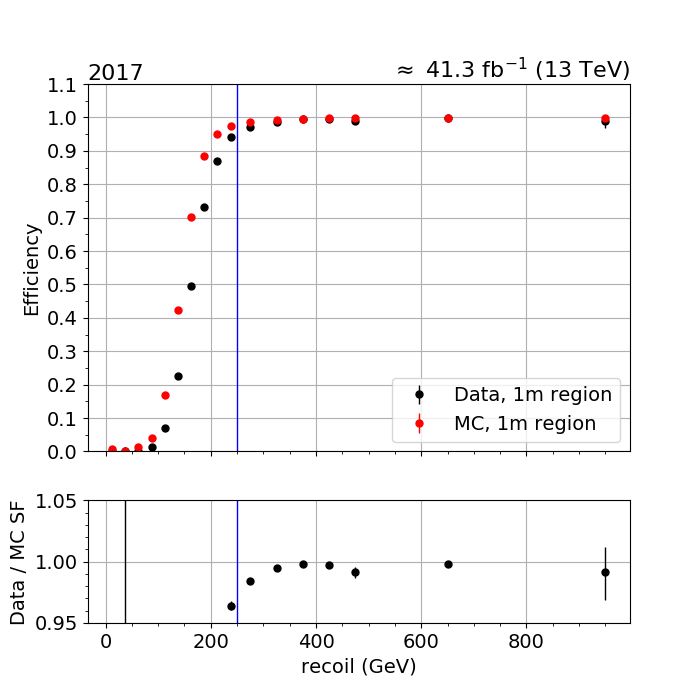
\includegraphics[width=0.49\textwidth]{fig/efficiency/trigger/met/recoil/data_mc_comparison_1m_2017_two_central_jets.png} \\
        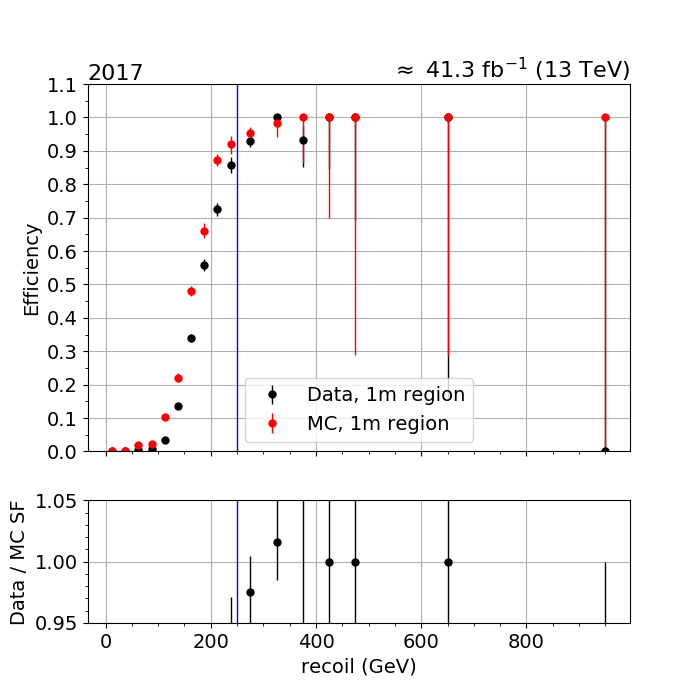
\includegraphics[width=0.49\textwidth]{fig/efficiency/trigger/met/recoil/data_mc_comparison_1m_2017_two_forward_jets.png}
    \end{center}
    \caption{MET trigger efficiency as a function of recoil in three categories: One forward jet and one central jet, two central jets and
            two forward jets. These results are obtained from 2017 data and MC samples with the selection of single muon events.} 
    \label{fig:eff_recoil_2017_1m}
\end{figure}

\begin{figure}[hbp]
    \begin{center}
        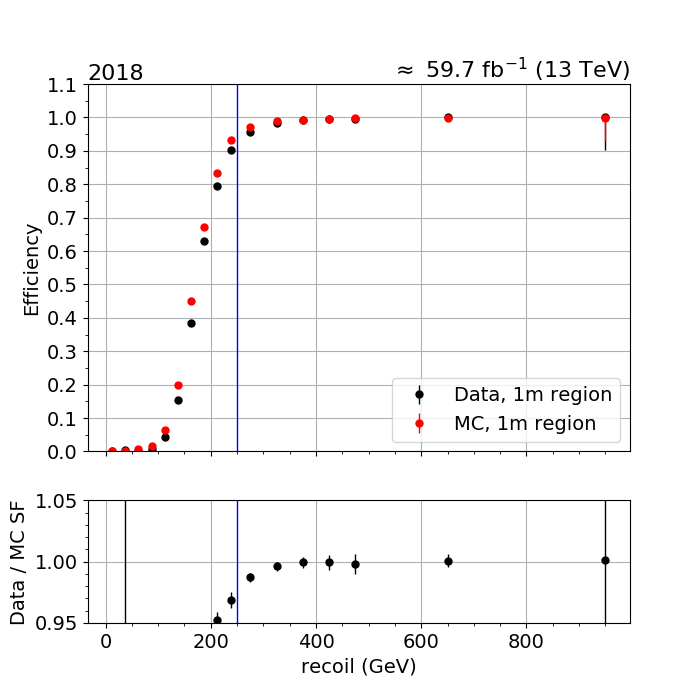
\includegraphics[width=0.49\textwidth]{fig/efficiency/trigger/met/recoil/data_mc_comparison_1m_2018_one_jet_forward_one_jet_central.png}
        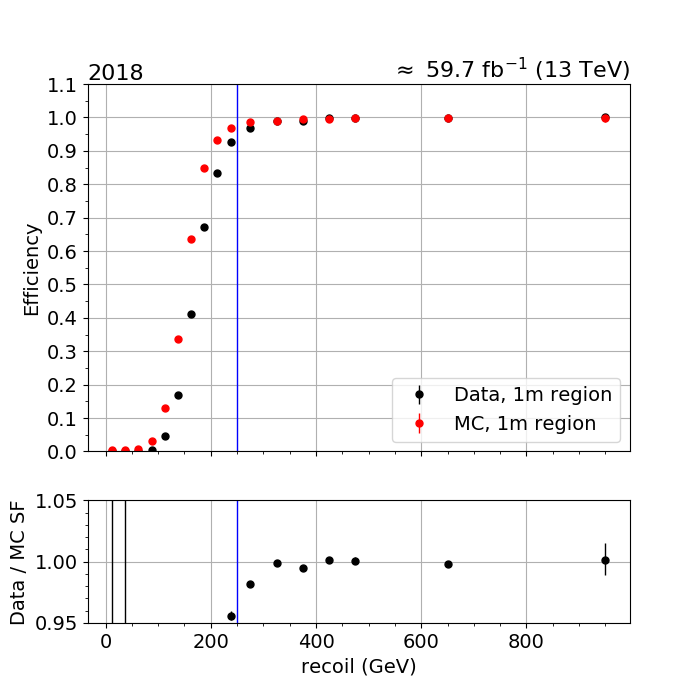
\includegraphics[width=0.49\textwidth]{fig/efficiency/trigger/met/recoil/data_mc_comparison_1m_2018_two_central_jets.png} \\
        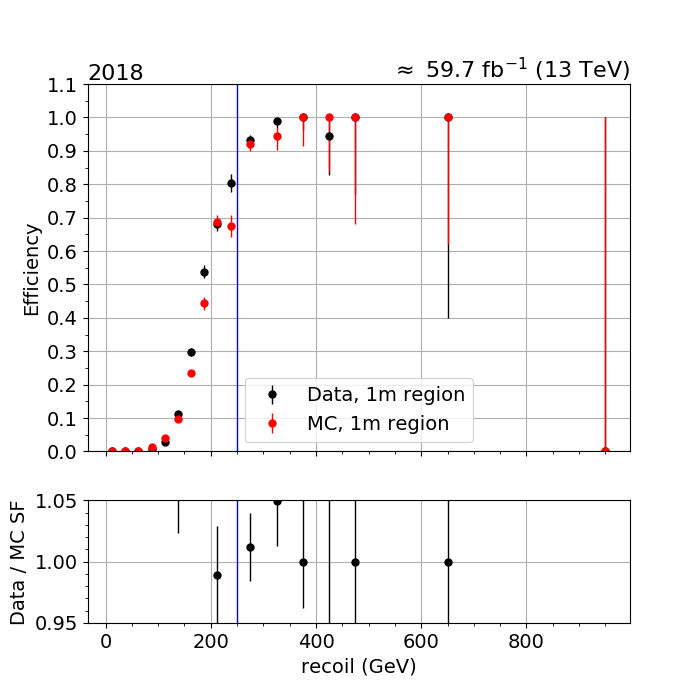
\includegraphics[width=0.49\textwidth]{fig/efficiency/trigger/met/recoil/data_mc_comparison_1m_2018_two_forward_jets.png}
    \end{center}
    \caption{MET trigger efficiency as a function of recoil in three categories: One forward jet and one central jet, two central jets and
            two forward jets. These results are obtained from 2018 data and MC samples with the selection of single muon events.}
    \label{fig:eff_recoil_2018_1m}
\end{figure}
